% Summary sys_impl here
The core of this system research thesis resides in the system implementation section which answers RQ1.

This section explains the method and the principles that will be used to carry out the software development process of adding support for \gls{HDFS} and \gls{HopsFS} to the delta-rs library. This section is divided into three sub sections: Development process, explaining the activities that will be carried out, Requirements, defining the functional and non-functional requirements of the system and Development environment, detailing the tools and resources that will be used during the development process.

\subsection{Development process}
The development process will follow an iterative and incremental development approach described in Figure \ref{fig:DevProcessRQ1}. This methodology will be applied as it allows flexibility, while creating incrementally a working system \cite{despa2014comparative}. This project, due to the need to work on \gls{HopsFS}, will require numerous interactions with \gls{HopsFS} maintainers (i.e. the industrial supervisor). This creates the need of a feedback loop, which will allow the system to fit all the requirements according to all stakeholders expectations.

As it can be noted from Figure \ref{fig:DevProcessRQ1}. Each step of this process is related to one of the goals (G1--G4) associated with RQ1 in Section \ref{sec:goals}.
The activities and the relationship between each activity and the associated goal(s) is here explained:
\begin{enumerate}
    \item \textbf{Identify problems collaboratively}: this activity solves partially G1--G2, as it is an initial system analysis, performed together with the industrial supervisor, who is knowledgeable on Hopsworks' infrastructure (in particular \gls{HopsFS}). This task fixes the initial requirements of the project and investigates what needs to be implemented at a high-level abstraction.
    \item \textbf{Analyse system}: this activity solves partially G1--G2 each time is re-iterated, as it performs a low level code based analysis of how the system works and what needs to be implemented to support \gls{HDFS} in delta-rs. This activity also starts an iterative loop that will end once the system fulfils the requirements described in Section \ref{subsec:requirements}.
    \item \textbf{Design software}: this activity solves partially G3, as the first part of the software development. In this activity the system analysed before is considered to design a solution.
    \item \textbf{Code software}: this activity solves partially G3, as the second part of the software development. In this activity the solution designed is coded.
    \item \textbf{Test system}: this activity solves partially G4, as first part of the tests performed to verify the solution validity, via unit tests. Failed unit tests will trigger a new development loop iteration, where this failure will be considered as first starting point in the system analysis.
    \item \textbf{Verify system integration}: this activity solves partially G4, as second part of the tests performed to verify the solution validity, via integration tests. Failed integration tests will trigger a new development loop iteration, where this failure will be considered as first starting point in the system analysis. On the other hand, if the integration test succeed, the loop will be restarted if the system does not yet fit a requirement, or finished if the system fulfils all requirements described in Section \ref{subsec:requirements}.
\end{enumerate}

This process will produce a final deliverable (D1), which is a Python wheel of the delta-rs library containing the support for \gls{HDFS} and \gls{HopsFS}.

\begin{figure}[!ht]
    \begin{center}
      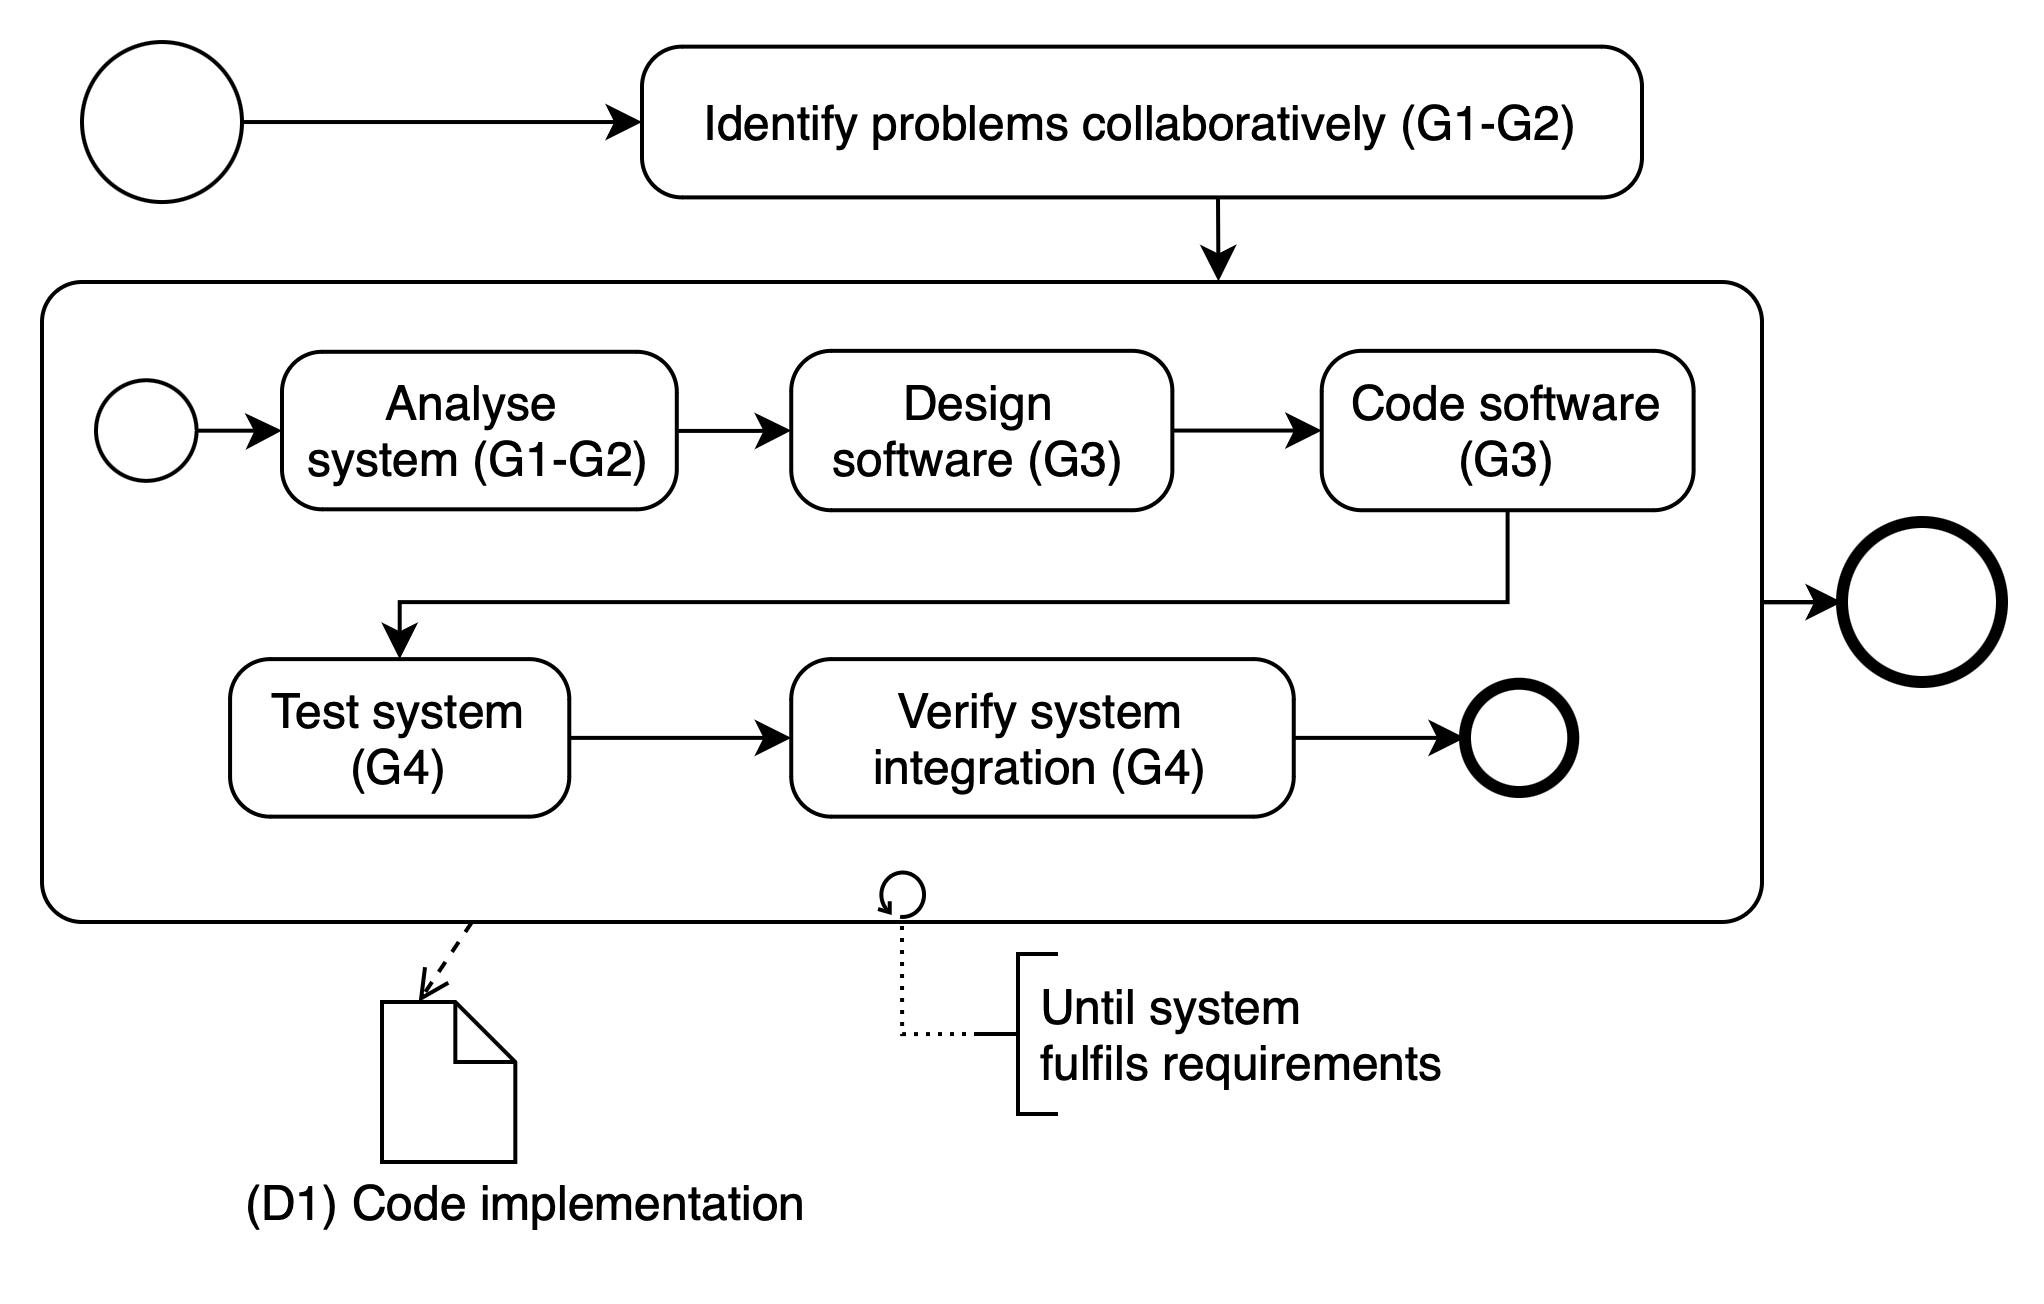
\includegraphics[width=\textwidth]{figures/3-method/research_process_rq1.png}
    \caption{\gls{BPMN} diagram of the System implementation process answering to RQ1. Each activity is associated with a specific Goal (\gls{G}). The process produces a deliverable (\gls{D}), in this case, a code implementation. The development loop iterates until the functional requirements (defined in Section \ref{subsec:requirements}) are fulfilled.}
    \label{fig:DevProcessRQ1}
    \end{center}
\end{figure}

\subsection{Requirements}
\label{subsec:requirements}
In the first steps of the system analysis, a series of requirements are defined in agreement with the industrial partner Hopsworks AB, to favor the creation of a solution that could be later used within the company, in a production environment. These are divided into two categories: functional and non-functional requirements. \\ The \textbf{functional requirements} are:
\begin{enumerate}
    \item \textbf{Write Delta Tables}: the solution should allow to write Delta Lake tables on \gls{HopsFS} via the delta-rs library.
    \item \textbf{Read Delta Tables}: the solution should allow to read Delta Lake tables on \gls{HopsFS} via the delta-rs library.
    \item \textbf{Communicate via TLS}: the solution should interact with \gls{HopsFS} via \gls{TLS} protocol version 1.2.
\end{enumerate}
The \textbf{non-functional requirements} are:
\begin{enumerate}
    \item \textbf{Consistent}: the solution should be consistent with the current open-source codebase used when appropriate.
    \item \textbf{Maintainable}: the solution should minimize the need for maintenance and support of the codebase in the future, minimizing changes to open-source code. When appropriate, the changes the solution introduces should be compatible with a future upstream merge to the open-source project modified.
    \item \textbf{Scalable}: the solution should be able to handle larger quantities of data (up to 100 GB) read or written on Delta Tables.
\end{enumerate}

\subsection{Development environment}
The system implementation will be developed by making use of several technologies, here categorized:
\begin{itemize}
    \item \textbf{Computing resources}: the system implementation will be developed in a remote environment accessed via \gls{SSH} from a computer terminal. This remote \gls{VM} is selected as mounting \gls{HopsFS} on a local machine is non-trivial and developing locally could result in inconsistencies when the solution is reproduced in a virtual environment.
    \item \textbf{Writing code}: the Vim \cite{WelcomeHomeVim} text editor is development tool of choice in combination with \gls{CoC} \cite{NeoclideCocnvim2024} providing language-aware autocompletion and rust-analyzer \cite{fannFannheywardCocrustanalyzer2024} access for on-code compiler errors. 
    \item \textbf{Libraries and dependencies}: for simpler development and tests reproducibility, the environment will be set in a Docker container \cite{DockerBuild0200}.
    \item \textbf{Code versioning and shared development}: GitHub \cite{GitHub} will be used for versioning, collaborating with open-source projects (e.g. delta-rs), and sharing the developed solution.
\end{itemize}

 